\documentclass[aspectratio=169, 10pt]{beamer}

\usetheme{CambridgeUS}
\usecolortheme{dolphin}
\setbeamertemplate{navigation symbols}{}
\setbeamertemplate{footline}[frame number]
\usefonttheme[onlymath]{serif}

\usepackage{booktabs}
\usepackage{listings}
\usepackage{xcolor}
\usepackage{tikz}

\lstset{
    basicstyle=\ttfamily\small,
    keywordstyle=\color{blue},
    commentstyle=\color{gray},
    backgroundcolor=\color{gray!10},
    frame=single,
    breaklines=true,
    language=Python
}
\setbeamertemplate{blocks}[rounded][shadow=true]
\setbeamercolor{block title}{bg=blue!10, fg=black}
\setbeamercolor{block body}{bg=blue!10, fg=black}

\title{Senior Health Workforce Analyst - Assignment}
\subtitle{Health Workforce Modelling}
\author{Jorge A. Garcia}
\date{October 19th, 2026}


\begin{document}


\begin{frame}
    \titlepage
\end{frame}


\begin{frame}{Outline}
    \tableofcontents
\end{frame}


\section{About me}
\begin{frame}{About me}
    Applied quantitative modeler with app development experience.
    \begin{itemize}
        \item Training:
        \begin{itemize}
            \item PhD. in Systems Design Engineering
            \item MSc. in Operations Research
            \item BSc. in Industrial Management
        \end{itemize}
        \vspace{0.3cm}
        \item My modelling experience:
        \begin{itemize}
            \item Decision models (optimization)
            \item Agent-based simulation
            \item Physics-based modelling
            \item Macroeconomic models
        \end{itemize}
    \end{itemize}
    \textcolor{blue}{\textbf{Goal:}}
    \begin{itemize}
        \item Apply quantitative modeling and data analytics to improve well-being of Ontarians.
        \item Learn and grow as a professional by taking on new challenges and responsibilities.
    \end{itemize}
\end{frame}


\section{Assignment \& Modelling Approach}
\begin{frame}{Assignment \& Modelling Approach}
    \begin{block}{Develop a quantitative model to forecast workforce supply and workforce requirements for \textbf{Registered Nurses} (RNs) in Ontario over the next 10 years.}
    \end{block}
    \vspace{0.5cm}
    \textbf{Modelling approach:}
    \begin{itemize}
        \item Start simple and enrich only if needed.
        \item Research or policy question being addressed (how a solution looks like?).
        \item Decision variables or policy instruments (what can be controlled?).
        \item Causal relationships between variables.
    \end{itemize}
    \vspace{0.2cm}
    \begin{center}
        \emph{There is no good solution to a badly posed problem.}
    \end{center}  
\end{frame}


\begin{frame}{Conceptual formulation}
    \centering
    \begin{tikzpicture}[
        box/.style={rectangle, rounded corners, draw=structure.fg, fill=structure.fg!10, minimum width=3.1cm, minimum height=1.4cm, align=center, font=\small},
        arr/.style={-latex, thick}]
        \node[box] (pop) at (0,2.) {Population [person]};
        \node[box] (dem) at (4.0,2.) {Healthcare service\\demand [hours/year]};
        \node[box] (gap) at (4.,0.) {Deficit/Surplus [hours/year]};
        \node[box] (sup) at (4, -2.) {Heathcare service\\supply [hours/year]};
        \node[box] (reg) at (8.,-2.) {RN [FTE]};
        \node[box] (rec) at (12,-2.) {Recruitment [FTE]};
        \draw[arr] (pop) -- (dem);
        \draw[arr] (dem) -- (gap);
        \draw[arr] (sup) -- (gap);
        \draw[arr] (reg) -- (sup);
        \draw[arr] (rec) -- (reg);
    \end{tikzpicture}
    \vspace{0.3cm}
    \begin{itemize}
        \item FTE: Full-time equivalent.
    \end{itemize}
\end{frame}


\begin{frame}{Model Decisions}
    \begin{itemize}
        \item Which variables are considered exogenous?
        \item Spatial and temporal granularity.
        \item Most appropriate model type, e.g.:
        \begin{itemize}
            \item System dynamics
            \item Time series
            \item Optimization
            \item Agent-based modelling
        \end{itemize}
        \item Model should drive data sources (rather than the other way around).
        \item Look for solutions in literature.
        \item Start with a simple model first.
    \end{itemize}
\end{frame}


\section{Demand-side Modelling}
\begin{frame}{Demand-side Modelling}
    \begin{itemize}
        \item Demand of healthcare services: $d_{t}$ [hours/time]
        \item $\alpha$: per capita demand for healthcare services [hours/(person time)]
        \item Population-driven demand:
        \begin{equation*}
            d_{t} = \alpha\ p_{t} \quad \forall t\quad\quad \text{[hours/time]}
        \end{equation*}
        \item Age-based demand: $d_{t} = \sum_{a} \alpha_{a}\ p_{a,t}$
        \item Specialty-based demand: $d_{t,s} = \sum_{a} \alpha_{a,s}\ p_{a,t}$
    \end{itemize}
\end{frame}

\begin{frame}{Population Modelling}
    \begin{itemize}
        \item Leslie (age-structured) model, in vector form:
        \begin{equation*}
            \mathbf{p}_{t+1} = \mathbf{L}\ \mathbf{p}_{t} + \mathbf{i}_{t} \quad \forall t
        \end{equation*}
        \item $\mathbf{p}_{t}$: population vector at time $t$.
        \item $\mathbf{L}$: Leslie matrix.
        \item $\mathbf{i}_{t}$: net immigration vector at time $t$ (major source of uncertainty).
    \end{itemize}

\end{frame}


\section{Supply-side Modelling}
\begin{frame}{Supply-side Modelling}
    \begin{itemize}
        \item Supply of healthcare services: $s_{t}$ [hours/time]
        \item $\beta_t$: per capita supply of healthcare services [hours/(FTE time)]
        \item $n_{t}$: number of healthcare professionals (FTE) at time $t$.
        \item Supply of healthcare services:
        \begin{equation*}
            s_{t} = \beta\ n_{t} \quad \forall t \quad\quad \text{[hours/time]}
        \end{equation*}
        \item Specialty-based supply: $s_{t,s} = \beta_{s}\ n_{s,t}$
    \end{itemize}
\end{frame}


\begin{frame}{Balance Surplus/Deficit}
    \begin{itemize}
        \item Balance of healthcare services:
        \begin{equation*}
            y_{t} = d_{t} - s_{t} \quad \forall t \quad\quad \text{[hours/time]}
        \end{equation*}
        \item Surplus: $y_{t}^{+} = \max(y_{t}, 0)$
        \item Deficit: $y_{t}^{-} = \max(-y_{t}, 0)$
    \end{itemize}
\end{frame}


\section{Optimal hiring policy model}
\begin{frame}{Optimal hiring policy model}
    \textbf{Decision variable} $x_{t}$: new RNs hired at time $t$.
    \vspace{0.2cm}
    \[
    \min_{x_{t}} \sum_{t=0}^{T} \lambda\ e^{-\delta t}\, y_{t}^{+} + \sum_{t=0}^{T} \mu\ e^{-\delta t}\, y_{t}^{-}
    \]
    s.t. 
    \begin{equation}
        d_{t} = \alpha_t\ p_{t}\quad \forall t
    \end{equation}

    \begin{equation}
        s_{t} = \beta_t\ n_{t}\quad \forall t
    \end{equation}

    \begin{equation}
        d_{t} - s_{t} = y_{t}^{+} - y_{t}^{-}  \quad \forall t
    \end{equation}

    \begin{equation}
        n_{t} = \gamma\ n_{t-1} + x_{t} \quad \forall t
    \end{equation}

    \begin{equation}
        x_{t}, y_{t}^{+}, y_{t}^{-} \ge 0 \quad \forall t
    \end{equation}
    
\end{frame}


\begin{frame}{Decision Support Tool}
    \begin{columns}[T]
        \column{0.50\textwidth}
        % Image
        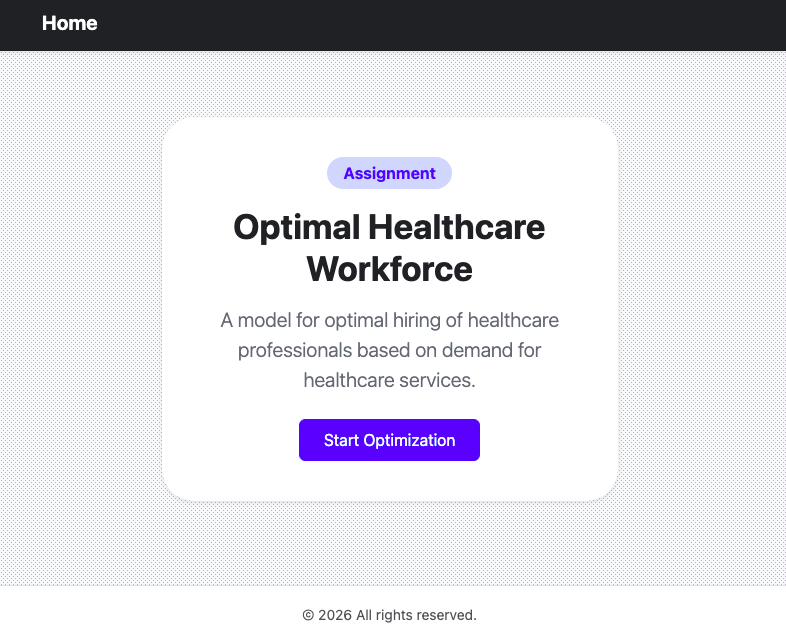
\includegraphics[width=\linewidth]{img/model.png}
        % Label
        \caption{Decision Support Tool: https://20.220.16.0/}
        \column{0.45\textwidth}
        \textbf{Development tools}
        \vspace{0.5cm}
        \begin{itemize}
            \item Model formulation: OR-Tools
            \item Application framework: Flask
            \item Infrastructure:
            \begin{itemize}
                \item Azure virtual machine (Ubuntu 24.04)
                \item Nginx, Gunicorn
            \end{itemize}
            \item \textcolor{blue}{Available at \url{https://20.220.16.0/}}
            \item Project repository: \url{https://github.com/jorge-antares/healthworkforce}
        \end{itemize}
    \end{columns}
\end{frame}


\begin{frame}{Extensions}
    \begin{itemize}
        \item Population's dynamics (Leslie model).
        \item CFacilities' capacity constraints: $n_{t} \le c_{t}$
        \item Recruitment sources $x_{t,s}$:
        \begin{itemize}
            \item domestic graduates
            \item international educated nurses
            \item re-entrants
        \end{itemize}
        \item Budget constraints on wages or recruitment.
        \item Bring economic theory: price elasticity of supply of nurses.
    \end{itemize}
\end{frame}


% ── Section c: Data ──────────────────────────────────────────────────────────
\section{Data limitations \& Uncertainty}
\begin{frame}{Data sources}
    \begin{itemize}
        \item Demographic data:
        \begin{itemize}
            \item Ministry of Finance population projections
            \item Statistics Canada
            \item CIHI health service utilization
        \end{itemize}
        \item Healthcare professionals data:
        \begin{itemize}
            \item College of Nurses of Ontario (CNO) registration statistics
            \item CIHI Nursing in Canada
            \item Program enrolment and graduation counts
        \end{itemize}
        \item Other sources as needed by the model
        \item \textbf{Privacy:} PII not needed for an aggregated model
        \item \textbf{Data gap:}
        \begin{itemize}
            \item Interpolation.
            \item Proportionality assumptions in the absence of detailed data.
            \item Use of proxy variables.
        \end{itemize}
    \end{itemize}
\end{frame}


\begin{frame}{Uncertainty Analysis}
    \textbf{Ways to address uncertainty:}
    \begin{enumerate}
        \item Probability distributions for key parameters or equations.
        \begin{itemize}
            \item Monte Carlo simulation.
            \item Expectation and Covariance matrix.
            \item Confidence intervals.
        \end{itemize}
        \item Error propagation analysis:
        \begin{itemize}
            \item Bounds on outputs.
        \end{itemize}
        \item Scenario analysis:
        \begin{itemize}
            \item Optimistic-case, pessimistic-case, and most-likely scenarios.
        \end{itemize}
        \item Sensitivity analysis:
        \begin{itemize}
            \item Assessing the impact of changes in key parameters on model outputs.
        \end{itemize}
    \end{enumerate}
\end{frame}


\section{Disclosure \& Summary}
\begin{frame}{Disclosure of Tools}
    Claude Sonnet 5.5 was used in the following tasks:
    \begin{itemize}
        \item Create HTML for user interface.
        \item Create initial presentation template.
        \item Code completion and debugging suggestions (VS Code).
    \end{itemize}
    \vspace{0.5cm}
    All LLM outputs were reviewed and edited.\\
    All model formulation and assumptions are 100\% the author's own.
\end{frame}


\begin{frame}{Summary}
    \begin{itemize}
        \item Use population as main driver.
        \item Start small and add complexity as needed.
        \item Construct a model that finds the least-cost to address supply-demand gaps.
        \item Address uncertainty through probability, error propagation, scenarios or sensitivity analysis.
    \end{itemize}
    \begin{center}
        \emph{All models are wrong, but some are useful.}
    \end{center}
    \vspace{0.5cm}
    \centering\Large Thank you --- questions?
\end{frame}

\end{document}
